\documentclass{article}
\usepackage[utf8]{inputenc}
\usepackage{amsfonts}
\usepackage{amssymb}
\usepackage{graphicx}
\usepackage{hyperref}
\usepackage{amsmath}
\usepackage{pgfplots}
\pgfplotsset{compat=1.18}
\usepackage[backend=biber, style=numeric]{biblatex}
\addbibresource{references.bib}
\usepackage{titlesec}
\titleformat{\subsection}[hang]{\normalfont\bfseries}{\thesubsection}{1em}{}
\usepackage{abstract}
\usepackage[labelformat=empty]{caption}

\begin{document}
\pagenumbering{gobble}
\begin{figure}
  \centering
  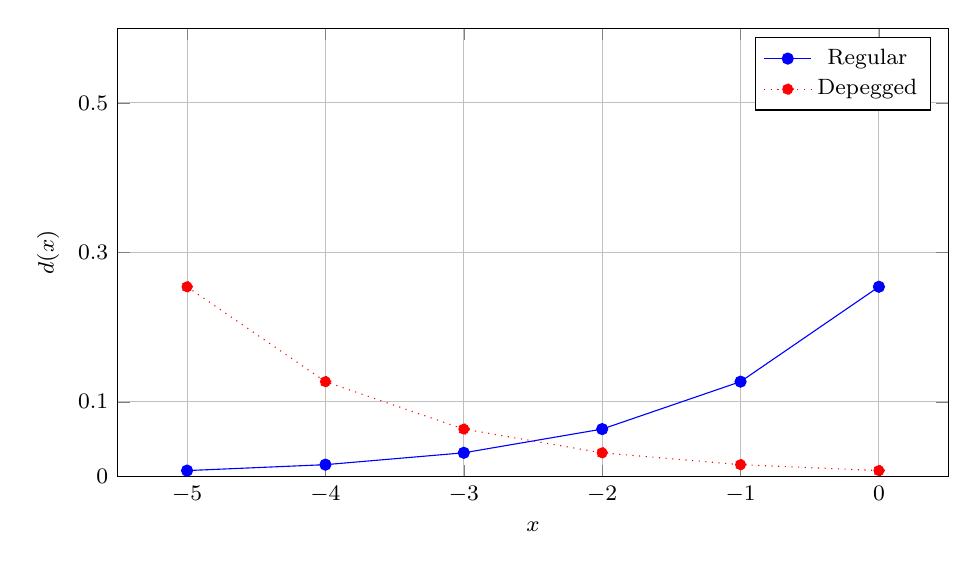
\begin{tikzpicture}
    \begin{axis}[
      xlabel={$x$},
      ylabel={$d(x)$},
      xmin=-5.5, xmax=0.5,
      ymin=0, ymax=0.6,
      xtick={-5,-4,-3,-2,-1,0},
      ytick={0,0.1,0.3,0.5},
      grid=major,
      width=\columnwidth,
      height=0.6\columnwidth,
      tick label style={font=\footnotesize},
      label style={font=\footnotesize},
      legend style={font=\footnotesize},
    ]
    
    \addplot[domain=-5:0, samples=6, color=blue, mark=*]{0.5 * 0.5^(-x)) / ((1 - 0.5^6) / (1 - 0.5))};
    \addlegendentry{Regular}
    \addplot[domain=-5:0, samples=6, color=red, mark=*, dotted]{0.5 * 0.5^(x+5)) / ((1 - 0.5^6) / (1 - 0.5))};
    \addlegendentry{Depegged}

    \end{axis}
  \end{tikzpicture}
  \caption{LDF for a high-risk stable pair (e.g. eETH/ETH) or yield pair (e.g. rETH/ETH) with "buy-the-dip" behavior}
  \label{fig:high_risk_stable}
\end{figure}

\end{document}